% !TEX root = ../main.tex

% Exercises section

\section{Summary statistics for categorical variables}

\begin{table}[H]
\centering
\begin{tabular}{|l|l|l|l|}
\hline
& treatment & & gender\\
\hline
intervention & 0.576 & male & 0.341 \\
\hline
control & 0.424 & female & 0.659\\
\hline
\end{tabular}
\caption{Summary statistics (proportion) for categorical variables}
\label{tab:summ.stat.cat}
\end{table}

\section{Additional Model Selection Tables and Plots}
\subsection{Covariate Selection for The Control Group}
\begin{table}[H]
\centering
\begin{tabular}{|l|l|l|}
\hline
& month & month + gender + education \\
\hline
month + gender & 0 & 0 \\
\hline
month + education & 0 & 0 \\
\hline
\end{tabular}
\caption{P values of Likelihood Ratio tests between models with different covariates under the control group}
\label{tab:model.comp.control.lrt}
\end{table}
\subsection{Random Effect Selection for The Control Group}
\begin{figure}[H]
\begin{subfigure}{.33\textwidth}
  \centering
  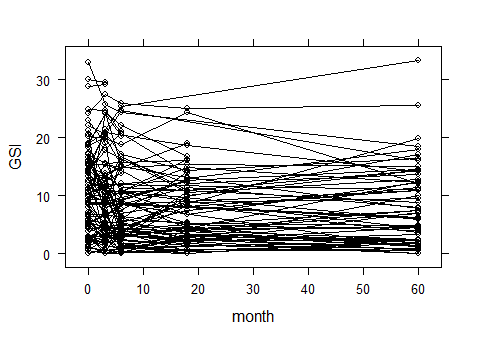
\includegraphics[width=1\linewidth]{../../plots/trellis_control.png}
  \caption{trellis plot of all subjects in the control group}
\end{subfigure}
\begin{subfigure}{.33\textwidth}
  \centering
  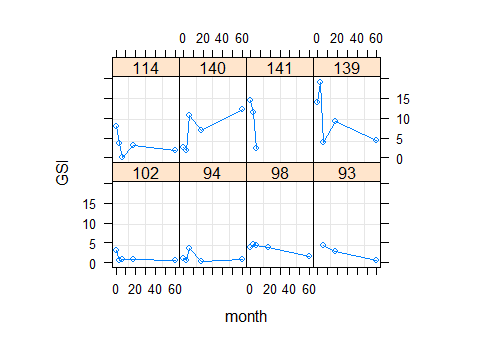
\includegraphics[width=1\linewidth]{../../plots/trellis_subset_control.png}
  \caption{trellis plot of randomly selected subjects}
\end{subfigure}
\begin{subfigure}{.33\textwidth}
  \centering
  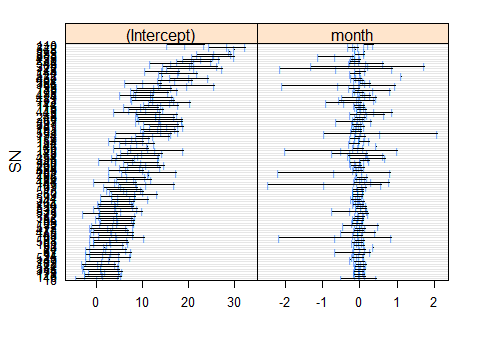
\includegraphics[width=1\linewidth]{../../plots/interval_control.png}
  \caption{confidence intervals of parameters from individual linear models}
\end{subfigure}
\caption{Diagnostic plots for selection of random effects for the control group}
\label{fig:diagnostic.control}
\end{figure}

\begin{table}[H]
\centering
\begin{tabular}{|l|l|l|}
\hline
& no mixed effect & intercept \\
\hline
intercept & 0 &/ \\
\hline
intercept + month &/ & 0.166 \\
\hline
intercept + gender &/ & 0.638 \\
\hline
intercept + education &/ & 0.981 \\
\hline
\end{tabular}
\caption{P values of Likelihood Ratio tests between models with different mixed effects under the control group}
\label{tab:model.comp.control.me.lrt}
\end{table}
\subsection{Covariate Selection for Both Groups Combined}
\begin{table}[H]
\centering
\begin{tabular}{|l|l|l|}
\hline
& treatment + month & treatment + month + gender + education \\
\hline
treatment + month + gender & 0 & 0 \\
\hline
treatment + month + education & 0 & 0 \\
\hline
\end{tabular}
\caption{P values of Likelihood Ratio tests between models with different covariates}
\label{tab:model.comp.lrt}
\end{table}
\subsection{Random Effect Selection for Both Groups Combined}
\begin{table}[H]
\centering
\begin{tabular}{|l|l|l|l|}
\hline
& no mixed effect & intercept & intercept + month \\
\hline
intercept & 0 &/ &/ \\
\hline
intercept + month &/ & 0.005 &/ \\
\hline
intercept + treatment &/ & 0.208 &/ \\
\hline
intercept + gender &/ & 0.487 &/ \\
\hline
intercept + education &/ & 0.999 &/ \\
\hline
intercept + month + treatment & /&/ & 0.343 \\
\hline
intercept + month + gender & /&/ & 0.690 \\
\hline
intercept + month + education & /&/ & 0.997 \\
\hline
\end{tabular}
\caption{P values of Likelihood Ratio tests between models with different mixed effects}
\label{tab:model.comp.me.lrt}
\end{table}

\section{Additional Assumption Check Plots}
\subsection{Control Group}
\begin{figure}[H]
\begin{subfigure}{.5\textwidth}
  \centering
  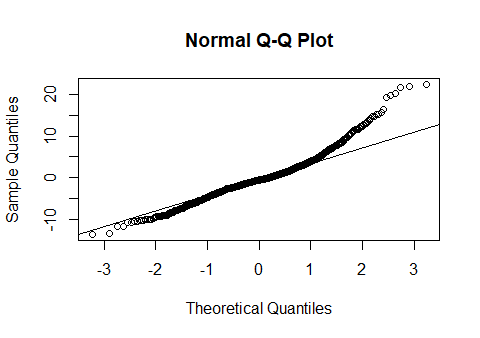
\includegraphics[width=1\linewidth]{../../plots/qq_residual_control.png}
  \caption{residual QQ plot}
\end{subfigure}
\begin{subfigure}{.5\textwidth}
  \centering
  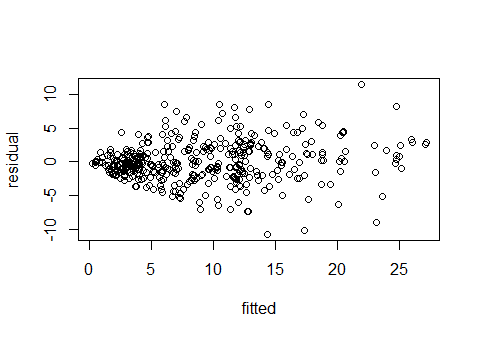
\includegraphics[width=1\linewidth]{../../plots/residual_control.png}
  \caption{fitted value vs. residual (t-test: 1, Wilcoxon: 0.501)}
\end{subfigure}
\caption{Visualizing the residuals of the LME model under the control group}
\label{fig:residual.control}
\end{figure}

\begin{figure}[H]
\centering
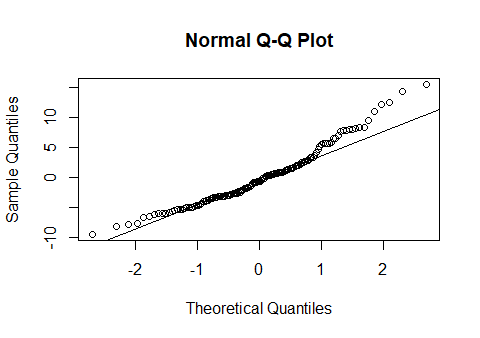
\includegraphics[width=0.5\linewidth]{../../plots/qq_intercept_treatment.png}
\caption{QQ plot for the random effects on the intercept (t-test: 1, Wilcoxon: 0.405)}
\label{fig:re.control}
\end{figure}
\subsection{Both Groups Combined}
\begin{figure}[H]
\begin{subfigure}{.5\textwidth}
  \centering
  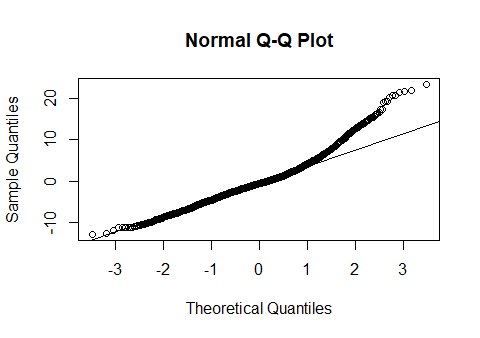
\includegraphics[width=1\linewidth]{../../plots/qq_residual.png}
  \caption{residual QQ plot}
\end{subfigure}
\begin{subfigure}{.5\textwidth}
  \centering
  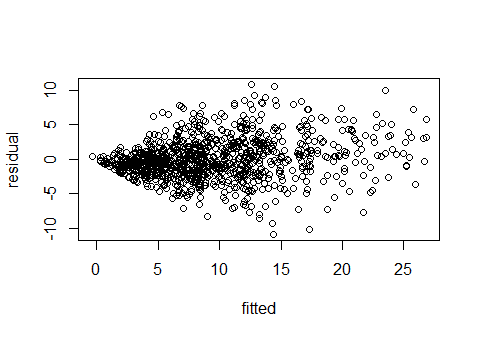
\includegraphics[width=1\linewidth]{../../plots/residual.png}
  \caption{fitted value vs. residual (t-test: 1, Wilcoxon: 0.143)}
\end{subfigure}
\caption{Visualizing the residuals of the LME model}
\label{fig:residual}
\end{figure}

\begin{figure}[H]
\begin{subfigure}{.5\textwidth}
  \centering
  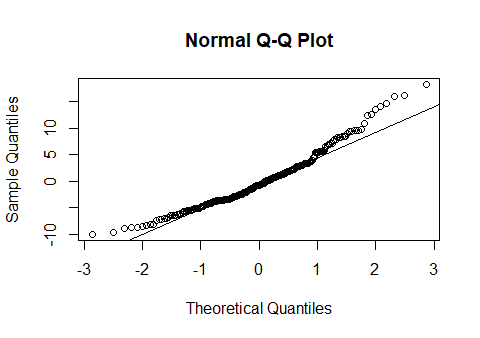
\includegraphics[width=1\linewidth]{../../plots/qq_intercept.png}
  \caption{QQ plot for the random effects on the intercept (t-test: 1, Wilcoxon: 0.207)}
\end{subfigure}
\begin{subfigure}{.5\textwidth}
  \centering
  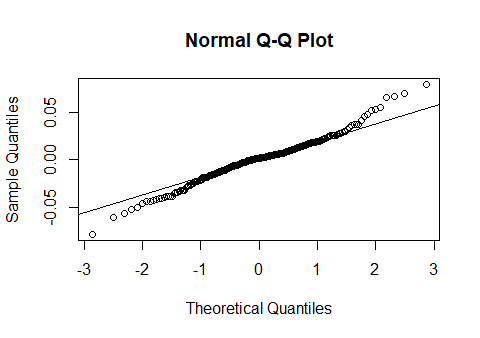
\includegraphics[width=1\linewidth]{../../plots/qq_slope.png}
  \caption{QQ plot for the random effects on the slope (t-test: 1, Wilcoxon: 0.786)}
\end{subfigure}
\caption{Visualizing the random effects}
\label{fig:re}
\end{figure}

\section{Pooled Analysis Results from Multiple Imputation}
\subsection{Intervention Group}
\begin{table}[H]
\centering
\begin{tabular}{|l|r|r|r|r|r|r|r|}
\hline
  & Estimate & Std.Error & t.value & df & P value \\
\hline
(Intercept) & 11.526 & 2.809 & 4.104 & 231.840 & 0.000 \\
\hline
month & -0.045 & 0.011 & -3.999 & 23.557 & 0.001 \\
\hline
gender2 & 2.734 & 0.968 & 2.824 & 239.207 & 0.005 \\
\hline
education & -0.222 & 0.199 & -1.115 & 107.937 & 0.268 \\
\hline
\end{tabular}
\caption{Output of pooled Linear Mixed Model under the intervention group}
\label{tab:lme.treatment.mi}
\end{table}

\begin{table}[H]
\centering
\begin{tabular}{|l|r|r|r|r|r|r|r|}
\hline
  & Estimate & Std.Error & t.value & df & P value \\
\hline
(Intercept) & 11.102 & 2.789 & 3.981 & 158.677 & 0.000 \\
\hline
month & -0.048 & 0.012 & -4.090 & 12.698 & 0.001 \\
\hline
gender2 & 2.733 & 0.942 & 2.902 & 355.509 & 0.004 \\
\hline
education & -0.188 & 0.198 & -0.947 & 78.666 & 0.347 \\
\hline
\end{tabular}
\caption{Output of pooled GEE model (naive) under the intervention group}
\label{tab:gee.treatment.mi.naive}
\end{table}

\begin{table}[H]
\centering
\begin{tabular}{|l|r|r|r|r|r|r|r|}
\hline
  & Estimate & Std.Error & t.value & df & P value \\
\hline
(Intercept) & 11.102 & 2.692 & 4.124 & 137.732 & 0.000 \\
\hline
month & -0.048 & 0.012 & -3.939 & 14.758 & 0.001 \\
\hline
gender2 & 2.733 & 0.908 & 3.009 & 307.277 & 0.003 \\
\hline
education & -0.188 & 0.191 & -0.985 & 67.256 & 0.328 \\
\hline
\end{tabular}
\caption{Output of pooled GEE model (robust) under the intervention group}
\label{tab:gee.treatment.mi.robust}
\end{table}

\subsection{Control Group}

\begin{table}[H]
\centering
\begin{tabular}{|l|r|r|r|r|r|r|r|}
\hline
  & Estimate & Std.Error & t.value & df & P value \\
\hline
(Intercept) & 19.695 & 4.011 & 4.910 & 1786.900 & 0.000 \\
\hline
month & -0.032 & 0.012 & -2.571 & 10.407 & 0.027 \\
\hline
gender2 & 2.277 & 1.315 & 1.732 & 5112.727 & 0.083 \\
\hline
education & -0.828 & 0.268 & -3.096 & 802.808 & 0.002 \\
\hline
\end{tabular}
\caption{Output of pooled Linear Mixed Model under the control group}
\label{tab:lme.control.mi}
\end{table}

\begin{table}[H]
\centering
\begin{tabular}{|l|r|r|r|r|r|r|r|}
\hline
  & Estimate & Std.Error & t.value & df & P value \\
\hline
(Intercept) & 20.598 & 4.119 & 5.000 & 208.709 & 0.000 \\
\hline
month & -0.027 & 0.014 & -1.999 & 14.750 & 0.064 \\
\hline
gender2 & 1.821 & 1.328 & 1.371 & 440.506 & 0.171 \\
\hline
education & -0.870 & 0.280 & -3.103 & 105.337 & 0.002 \\
\hline
\end{tabular}
\caption{Output of pooled GEE model (naive) under the control group}
\label{tab:gee.control.mi.naive}
\end{table}

\begin{table}[H]
\centering
\begin{tabular}{|l|r|r|r|r|r|r|r|}
\hline
  & Estimate & Std.Error & t.value & df & P value \\
\hline
(Intercept) & 20.598 & 3.695 & 5.575 & 135.062 & 0.000 \\
\hline
month & -0.027 & 0.014 & -1.949 & 16.329 & 0.069 \\
\hline
gender2 & 1.821 & 1.302 & 1.399 & 406.382 & 0.163 \\
\hline
education & -0.870 & 0.242 & -3.590 & 58.813 & 0.001 \\
\hline
\end{tabular}
\caption{Output of pooled GEE model (robust) under the control group}
\label{tab:gee.control.mi.robust}
\end{table}

\subsection{Both Groups Combined}

\begin{table}[H]
\centering
\begin{tabular}{|l|r|r|r|r|r|r|r|}
\hline
  & Estimate & Std.Error & t.value & df & P value\\
\hline
(Intercept) & 14.858 & 2.439 & 6.091 & 135.244 & 0.000 \\
\hline
treatment2 & -0.171 & 0.733 & -0.234 & 802.931 & 0.815 \\
\hline
month & -0.039 & 0.009 & -4.167 & 15.060 & 0.001 \\
\hline
gender2 & 2.604 & 0.829 & 3.139 & 108.962 & 0.002 \\
\hline
education & -0.467 & 0.172 & -2.715 & 58.348 & 0.009 \\
\hline
\end{tabular}
\caption{Output of pooled Linear Mixed Model}
\label{tab:lme.mi}
\end{table}

\begin{table}[H]
\centering
\begin{tabular}{|l|r|r|r|r|r|r|r|}
\hline
  & Estimate & Std.Error & t.value & df & P value\\
\hline
(Intercept) & 14.644 & 2.449 & 5.980 & 98.809 & 0.000 \\
\hline
treatment2 & -0.223 & 0.724 & -0.307 & 832.892 & 0.759 \\
\hline
month & -0.039 & 0.011 & -3.678 & 8.707 & 0.005 \\
\hline
gender2 & 2.591 & 0.810 & 3.197 & 140.824 & 0.002 \\
\hline
education & -0.446 & 0.173 & -2.582 & 48.524 & 0.013 \\
\hline
\end{tabular}
\caption{Output of pooled GEE model (naive)}
\label{tab:gee.mi.naive}
\end{table}

\begin{table}[H]
\centering
\begin{tabular}{|l|r|r|r|r|r|r|r|}
\hline
  & Estimate & Std.Error & t.value & df & P value\\
\hline
(Intercept) & 14.644 & 2.356 & 6.215 & 84.692 & 0.000 \\
\hline
treatment2 & -0.223 & 0.742 & -0.300 & 917.614 & 0.764 \\
\hline
month & -0.039 & 0.011 & -3.594 & 9.554 & 0.005 \\
\hline
gender2 & 2.591 & 0.786 & 3.298 & 124.401 & 0.001 \\
\hline
education & -0.446 & 0.168 & -2.655 & 43.400 & 0.011 \\
\hline
\end{tabular}
\caption{Output of pooled GEE model (robust)}
\label{tab:gee.mi.robust}
\end{table}

\section{R Code Excerpt (Intervention Group)}
\lstinputlisting[language=R]{C:/2020W2/STAT550/individualproject/excerpt.R}